\chapter{Porównanie dostępnych narzędzi}\label{chap:tools}
W tym rozdziale zostają opisane i porównane narzędzia wykorzystywane w czasie procesu budowy i rozwoju aplikacji stworzonych w języku Elm oraz kombinacji Reacta i Reduxa. Głównymi elementami na których jest skupiony rozdział są menedżery pakietów, narzędzia do statycznej analizy kodu oraz jego formatowania, a także narzędzia do monitorowania stanu w czasie działania aplikacji.

\section{Biblioteki i menedżery pakietów}
Ponieważ React, poza swoją specjalną składnią do opisywania komponentów widoku, składa się z~kodu JavaScriptu, to wykorzystywanym przez niego menedżerem pakietów jest npm. 

npm jest to menedżer pakietów dla języka JavaScript. Obecnie jest on także największym rejestrem oprogramowania, zawierający ponad 600 tysięcy pakietów kodu JavaScriptu z około 3 miliardami pobrań w ciągu jednego tygodnia \cite{whatIsNpm}. Menedżer pakietów npm składa się tak naprawdę z sieciowej bazy danych zawierającej publiczne, jak i płatne pakiety JavaScript oraz z klienta używanego w środowisku konsolowym. Rejest jest dostępny za pośrednictwem konsoli, a dostępne pakiety można przeglądać i~wyszukiwać za pomocą strony internetowej. 

Wszystkie pakiety instalowane w danej lokalizacji są zapisywane w specjalnym katalogu \lstinline{node_modules}, w którym znajdują się wszystkie zainstalowane pakiety oraz zależności wymagane do ich działania. Instalacja pakietów odbywa się poprzez polecenie \lstinline{npm install <nazwa_pakietu>}, co spowoduje instalację lokalną biblioteki w aktualnym folderze do katalogu \lstinline{node_modules}. Pakiet może być także zainstalowany globalnie, co umożliwia użycie go w dowolnym projekcie bez konieczności posiadania go bezpośrednio w każdym z nich.

Aby ułatwić zarządzanie lokalnie zainstalowanych pakietów, używany jest specjalny plik konfiguracyjny \lstinline{package.json}. Plik ten zawiera listę pakietów, od których zależy projekt, dla każdego z nich określając wersję pakietu, z których powinien korzystać projekt. Pozwala to na łatwe odtworzenie kompilacji, co znacznie upraszcza dzielenie kodu między programistami. Przykładową formę pliku można zobaczyć na fragmencie \ref{listing:package}.

\begin{minipage}{\linewidth}
\begin{lstlisting}[caption=Przykładowy plik package.json, tabsize=2, label=listing:package]
{
	"name": "elm-webpack-starter",
	"description": "Webpack setup for writing Elm apps",
	"version": "0.8.6",
	"license": "MIT",
	"author": "Peter Morawiec",
	"repository": {
		"type": "git",
		"url": "https://github.com/oszust002/elm-webpack-starter"
	},
	"scripts": {
		"start": "elm-css src/elm/Stylesheets.elm",
		"prebuild": "rimraf dist",
		"build": "webpack",
		"reinstall": "npm i && elm package install"
	},
	"devDependencies": {
		"autoprefixer": "^6.7.7",
		"elm-css": "^0.6.1"
	}
}
\end{lstlisting}
\end{minipage}
Aby uzyskać domyślny wersję pliku używa się komendy \lstinline{npm init --yes}, która na podstawie informacji zawartych w folderze projektu wygeneruje podstawowy plik konfiguracyjny zawierający pola:
\begin{itemize}
	\item name -- nazwa projektu. Domyślną wartością jest nazwa aktualnego katalogu
	\item version -- wersja projektu. Domyślnie zawsze jest to 1.0.0
	\item descripton -- krótki opis projektu. W przypadku istnienia pliku readme pobierana jest pierwsza linijka tego pliku, w przeciwnym wypadku jest tutaj wpisywany pusty ciąg znaków
	\item main -- wskazanie lokalizacji głównego pliku projektu. Domyślnie zawsze wskazywany jest plik \lstinline{index.js}
	\item scripts -- lista skryptów, które można wykonać przy pomocy polecenia \lstinline{npm run <nazwa_skryptu>}. Domyślnie tworzony jest pusty skrypt test
	\item keywords -- lista słów kluczowych, umożliwiająca znalezienie pakietu w rejestrze. Domyślnie jest ona pusta
	\item author -- informacje na tematu autora pakietu. Domyślnie pole to jest pustym ciągiem znaków
	\item license -- rodzaj licencji, która obejmuje pakiet. Domyślnie wpisywana jest licencja ISC.
\end{itemize}

Menedżer pakietów npm jest także często wykorzystywany przy tworzeniu projektów stworzonych w języku Elm. Jest on głównie wykorzystywany do instalowania pakietów pomocniczych, które pozwalają na interakcję z kodem Elma, taką jak generowanie kodu. Jednak projekty stworzone w języku Elm korzystają głównie z menedżera pakietów elm-package stworzonego przez twórcę Elma. Podobnie jak w~przypadku npm-a, elm-package składa się tak naprawdę na konsolowy interfejs służący do zarządzania pakietami w projekcie, oraz strony internetowej pozwalającej na przeglądanie poszczególnych pakietów \cite{elmPackage}. Niestety z powodu krótkiego istnienia języka oraz samego menedżera, liczba dostępnych pakietów, wynosząca niewiele ponad 1000 bibliotek, jest nieporównywalnie mała w stosunku do ilości pakietów wpisanych w rejestr npm-a. 

Podobnie jak w przypadku npm-a, menedżer pakietów dla języka Elm pozwala na łatwe zarządzanie pakietami wykorzystywanymi w projekcie. Odpowiednikiem pliku konfiguracyjnego jest tutaj plik \lstinline{elm-package.json}, znajdujący się w głównym katalogu projektu. Nowy plik konfiguracyjny jest tworzony w trakcie instalowania pierwszej biblioteki. Instalacja odbywa się za pomocą polecenia \lstinline{elm-package install <autor>/<nazwa_biblioteki> <wersja>}. Wymaganie autora biblioteki jest spowodowane tym, że menedżer pakietów dla języka Elm jest w tej chwili ograniczony wyłącznie do repozytoriów znajdujących się w serwisie GitHub. Wersja jest natomiast argumentem opcjonalnym, w przypadku niepodania go zostanie zainstalowana najnowsza wersja pakietu.
\begin{minipage}{\linewidth}
\begin{lstlisting}[caption=Przykładowy plik elm-package.json, tabsize=2, label=listing:elmPackage]
{
	"version": "1.0.0",
	"summary": "Example using `elm-webpack-loader`.",
	"repository": "https://github.com/moarwick/elm-webpack-starter.git",
	"license": "MIT",
	"source-directories": [ "src/elm" ],
	"exposed-modules": [],
	"dependencies": {
		"debois/elm-mdl": "8.1.0 <= v < 9.0.0",
		"elm-lang/core": "5.0.0 <= v < 6.0.0",
		"elm-lang/html": "2.0.0 <= v < 3.0.0",
		"rtfeldman/elm-css": "11.2.0 <= v < 12.0.0",
		"rtfeldman/elm-css-helpers": "2.1.0 <= v < 3.0.0"
	},
	"elm-version": "0.18.0 <= v < 0.19.0",
}
\end{lstlisting}
\end{minipage}
Na fragmencie \ref{listing:elmPackage} można zobaczyć przykładową formę pliku \lstinline{elm-package.json}. Analogicznie jak w~przypadku npm-a, znajdują się tutaj informacja na temat wersji projektu, krótkie podsumowanie, rodzaj licencji, czy w końcu lista pakietów wykorzystywanych w projekcie. Niestety pakiety mogą być instalowane tylko w sposób lokalny. To, co odróżnia zawartość pliku konfiguracyjnego dla elm-package od konfiguracji pakietów w npm-ie, jest między innymi brak nazwy pakietu, zastąpione adresem do repozytorium zawierającego paczkę. Nie ma tutaj także możliwości uruchamiania własnych skryptów, które mogłyby uprościć proces zarządzania aplikacją. Dodatkowo na końcu pliku znajduje się wersja wykorzystywanej implementacji języka Elm. Dzięki temu menedżer pakietów jest w stanie ustalić, które wersje bibliotek są kompatybilne z wykorzystaną wersją języka.

W przypadku pakietów języka Elm, wersje są istotnym aspektem ze względu na funkcjonalność obliczania zmian. Każda z bibliotek posiada wersję składającą się z trzech części: MAJOR, MINOR oraz PATCH. W pierwszym przypadku mamy do czynienia ze znaczną zmianą API, w której istniejące funkcjonalności zostały zmienione lub usunięte. W przypadku zmiany MINOR dodane zostały nowe funkcjonalności, bez wprowadzania jakichkolwiek zmian do już istniejących. Zmiana PATCH odpowiada za drobne poprawki nie zmieniające w żaden sposób API biblioteki. Menedżer pakietów przy pomocy polecenia \lstinline{elm-package bump} potrafi porównać wersję aktualną pakietu z wersją opublikowaną i na podstawie różnic automatycznie podnieść wersję aplikacji. W bardzo podobny sposób użytkownik, który chce sprawdzić różnice między konkretnymi wersjami danej biblioteki jest w stanie przy pomocy polecenia \lstinline{elm-package diff <autor>/<nazwa> <wersja1> <wersja2>} sprawdzić jakie dokładnie nastąpiły zmiany. Jest to możliwe dzięki wymuszeniu na osobach publikujących dodawania dokumentacji do projektu, która opisuje każdą z udostępnionych funkcjonalności. Obliczanie i sprawdzanie zmian pomiędzy wersjami to funkcja, która pomaga w zarządzaniu wykorzystywanymi wersjami bibliotek, a która niestety nie jest dostępna w przypadku menedżera pakietów npm.

\section{Statyczna analiza i formatowanie kodu}
W przypadku języka JavaScript narzędziami, które odpowiadają za statyczną analizę i formatowanie kodu źródłowego, są tak zwane lintery. Potrafią one wykryć potencjalne błędy, a także kod, który według zasad zdefiniowanych w danym linterze, jest trudny do utrzymania. Przykładami linterów są między innymi JSLint, JSHint, czy w końcu obecnie chyba najpopularniejszy z nich, ESLint. Ze względu na to, że ESLint jest jedynym narzędziem wspierającym składnię JSX wykorzystaną w React'cie, skupię się głównie na nim. Po stronie języka Elm trzeba rozróżnić dwa oddzielne narzędzia. Pierwszym jest po prostu kompilator Elma, który dzięki właściwościom języka potrafi przeprowadzać statyczną analizę kodu w czasie kompilacji. Drugim narzędziem natomiast jest pakiet elm-format, formatujący kod na podstawie oficjalnego przewodnika z zasadami poprawnego formatowania kodu w języku Elm~\cite{elmStyleGuide}. 

ESLint bazujący na wbudowanych zasadach poprawnego tworzenia kodu JavaScriptu potrafi wykryć błędy, które mogłyby doprowadzić do pojawienia się wyjątków po uruchomieniu aplikacji w przeglądarce. Na podstawie tychże zasad potrafi także ocenić jakość kodu stworzonego przez programistę i~zwrócić informację o tym, w jaki sposób można ten kod poprawić \cite{ESLint}. ESLint oferuje także elastyczność co do wykorzystywanych reguł. W każdej chwili, jeżeli programista nie chce, żeby dany fragment kodu był analizowany przez linter w kontekście jakiejś reguły, może wyłączyć ją za pomocą specjalnych przypisów dodanych w komentarzach. Pod tym względem zarówno kompilator języka Elm, jak i~biblioteka elm-format są o wiele bardziej restrykcyjne. Kompilator, przeprowadzając statyczną analizę kodu w czasie kompilacji, nie pozwoli na uruchomienie programu do momentu, w którym programista nie poprawi wskazanych fragmentów kodu. W przypadku elm-format sytuacja wygląda nieco inaczej. Biblioteka ta, zamiast analizować kod i wskazując niepoprawne miejsca programiście, automatycznie sama poprawia kod, opierając się na regułach dotyczących stylu opisanych w dokumentacji języka Elm \cite{elmStyleGuide}. Programista nie może zmienić reguł używanych przez elm-format, co narzuca wymóg tworzenia kodu w~jeden uniwersalny sposób.

O ile oczywistym jest to, że kompilator Elma jest narzędziem wbudowanym w język Elm, o tyle zarówno użycie ESLinta i biblioteki elm-format wymaga zewnętrznej konfiguracji. W obu przypadkach konfiguracja zaczyna się od zainstalowania bibliotek przy pomocy menedżera pakietów npm. Po tym kroku, biblioteka elm-format jest już gotowa do użycia, natomiast ESLint wymaga dodatkowej konfiguracji dla każdego projektu w którym ma być użyty. Odbywa się to za pomocą komendy \lstinline{eslint --init} generującej plik konfiguracyjny zawierający konfigurację jakie reguły mają zostać użyte w trakcie analizy kodu.

Choć doświadczeni programiści tworzący aplikacje internetowe używają powyższych narzędzi nawet o tym nie myśląc, to w przypadku osób zaczynających dopiero przygodę z programowaniem aplikacji internetowych, zdarza się nie wiedzieć o ich istnieniu. W przypadku języka Elm tracimy wyłącznie analizę i poprawę formatowania kodu. Kompilator jest wbudowanym narzędziem, które zawsze w przypadku błędów w kodzie, jest w stanie je znaleźć i przekazać użytkownikowi. Niestety w przypadku braku użycia ESLinta jesteśmy narażeni na wystąpienie błędów w trakcie działania programu. Aby pokazać na czym polega różnica, można rozważyć błąd, który jest popełniany bardzo często przez wielu programistów. Takim błędem są literówki. Niech w obu przypadkach występuje pole o nazwie \lstinline{fatalError}. W kontekście języka Elm pole to będzie częścią struktury modelu aplikacji, natomiast w implementacji Reacta będzie to jedno z pól właściwości dla komponentu.

\begin{minipage}{.45\textwidth}
	\begin{lstlisting}[style=elm-style,label = listing:elmmodel, numbers=left, stepnumber=1]
	type alias Model =
		{ field: String
		, fatalError: Bool
		}
	\end{lstlisting}
\end{minipage}\hfill
\begin{minipage}{.45\textwidth}
	\begin{lstlisting}[style=JavaScript,firstnumber=1,label=listing:reactprops]
	static propTypes = {
		field: React.PropTypes.string,
		fatalError: React.PropTypes.bool,
	};
	\end{lstlisting}
\end{minipage}

Aby wywołać błąd w obu przypadkach wystarczy odwołać się do pola \lstinline{fatalError}, jednak używając błędnie wpisanej nazwy \lstinline{fatalEror}. W przypadku implementacji w języku Elm, błąd zostanie wykryty już w czasie kompilacji. Rysunek \ref{fig:elmError} pokazuje komunikat wyświetlony przez kompilator, w~którym poza dokładnym miejscem wystąpienia błędu, programista otrzymuje podpowiedź o prawdopodobnej nazwie pola, której chciał użyć. Implementacja Reacta, w której nie skorzystano z ESLinta uruchomiła się nie podając żadnych komunikatów o błędach. Dopiero po wejściu na stronę internetową programista jest w stanie zauważyć że widok nie został załadowany, a sama informacja o występującym błędzie jest widoczna dopiero w konsoli deweloperskiej przeglądarki. Komunikat pokazany na rysunku~\ref{fig:reactError} jest stosem opisującym błąd, który mówi wprawdzie o nieistniejącej właściwości, jednak rozmiar komunikatu sprawia, że jest on mało czytelny. W przypadku większej ilości błędów, które mogą być dużo bardziej skomplikowane, programista może spędzić więcej czasu na szukaniu informacji o faktycznym błędzie, niż na samej jego poprawie.

\begin{figure}[h]
	\centering
	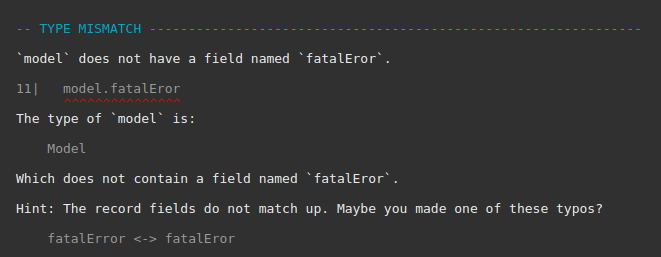
\includegraphics[width=0.9\textwidth]{images/elm_error}
	\caption{Komunikat kompilatora o nieistniejącym polu}
	\label{fig:elmError}
\end{figure}

\begin{figure}[h]
	\centering
	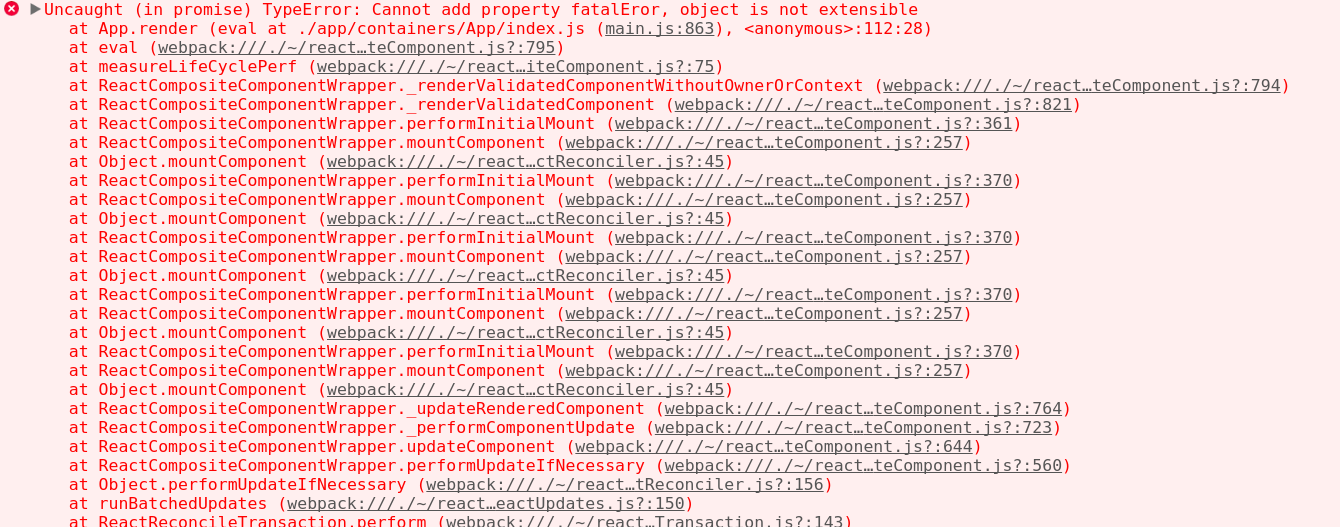
\includegraphics[width=0.9\textwidth]{images/react_error}
	\caption{Komunikat o błędzie w konsoli deweloperskiej przeglądarki Google Chrome}
	\label{fig:reactError}
\end{figure}

\section{Debugger języka Elm i Redux DevTools}
Sposób przepływu i aktualizacji danych w języku Elm i bibliotece Redux opiera się na komunikatach. Każda akcja, która w jakiś sposób modyfikuje stan aplikacji, jest odwzorowywana przez pojedynczą wiadomość. Takie podejście pozwala na łatwe monitorowanie stanu w czasie. Tym właśnie zajmują się narzędzia takie jak wbudowany w implementację języka Elm debugger oraz Redux DevTools.

Aby móc skorzystać z debuggera języka Elm, należy uruchomić program w trybie debug. To sprawia, że w prawym dolnym rogu widok aplikacji internetowej zostaje dołączona zakładka, która po kliknięciu przedstawia widok pokazany na rysunku \ref{fig:elmDebugger}. Po lewej stronie okna znajduje się lista wiadomości wysłanych od początku uruchomienia aplikacji w przeglądarce. Prawa strona natomiast prezentuje strukturę stanu w danym momencie działania aplikacji. Po kliknięciu jednej z wiadomości można zauważyć, że~z~prawej strony został pokazany stan z momentu tuż po zaaplikowaniu aktualizacji danych na podstawie tejże wiadomości. Stan ten jest aplikowany także do widoku, przez co programista jest w stanie zobaczyć, jak zmienia się widok w momencie wystąpienia konkretnego rodzaju komunikatu. Dodatkowo cały proces działania aplikacji można zapisać w formie pliku, co jest ogromnym ułatwieniem w procesie naprawiania błędów. Programista odpowiadający za dany fragment kodu ma możliwość wtedy wczytać cały proces z przekazanego mu pliku, dokładnie odtworzyć błąd, który wystąpił i znaleźć jego przyczynę.
\begin{figure}[h]
	\centering
	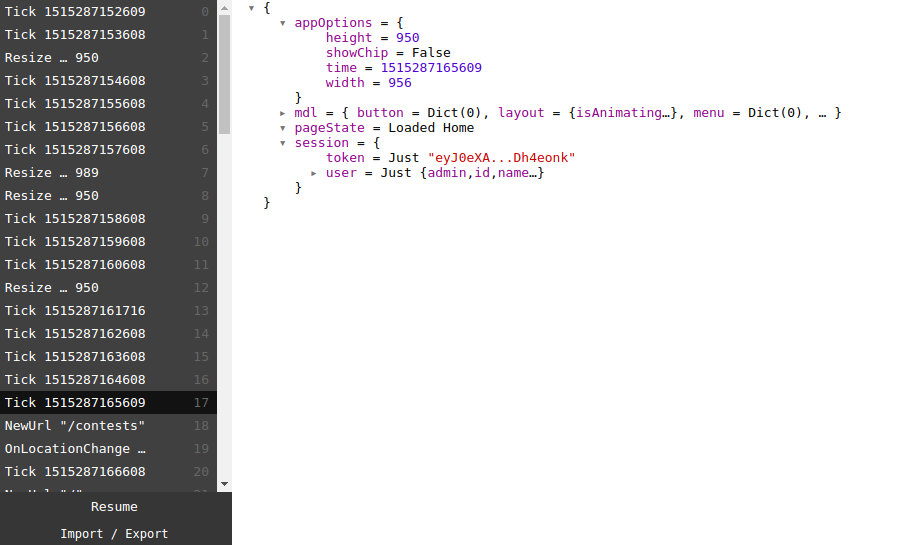
\includegraphics[width=\textwidth]{images/elm_debugger}
	\caption{Okno debuggera języka Elm}
	\label{fig:elmDebugger}
\end{figure}

Redux DevTools jest dodatkiem do przeglądarek takich jak Google Chrome czy Mozilla Firefox. Poza zainstalowaniem dodatku w przeglądarce należy dodać odpowiednie opcje we fragmencie kodu, w którym tworzony jest, przy pomocy funkcji Reduxa, stan całej aplikacji. Następnie po uruchomieniu aplikacji w narzędziach deweloperskich przeglądarki należy wejść w zakładkę \textit{Redux}, która pokaże nam okno pokazane na rysunku \ref{fig:reduxDevTools}. Od razu można zauważyć, że podobnie jak w~debuggerze Elma, po lewej stronie znajdują się akcje odpowiadające za aktualizację stanu, natomiast po prawej widać stan aplikacji w wybranym momencie. Można też tutaj, podobnie jak w debuggerze, zapisywać i wczytywać proces działania aplikacji. Jednak widać także, że Redux DevTools jest narzędziem znacznie bardziej rozbudowanym. Użytkownik może wybrać jeden z trzech sposobów wyświetlania drzewa stanu: jako drzewo danych tekstowych, wykres wizualizujący strukturę drzewa oraz bezpośrednie dane bez żadnej modyfikacji wizualnej. Poza widokiem stanu w danym momencie można także sprawdzić zawartość akcji, jaka została wtedy wysłana, a także spojrzeć na zmiany wprowadzone do stanu w skutek obsłużenia przychodzącej akcji. Dodatkową opcją jest też suwak pozwalający na przeglądanie zmian stanu w formie osi czasu. To, czego brakuje w narzędziu React DevTools w porównaniu do debuggera języka Elm to wizualizacja zmian na widoku aplikacji. Ponieważ narzędzie to jest tylko dodatkiem do przeglądarki, to nie ma ono bezpośredniego wpływu na widok aplikacji.

\begin{figure}[h]
	\centering
	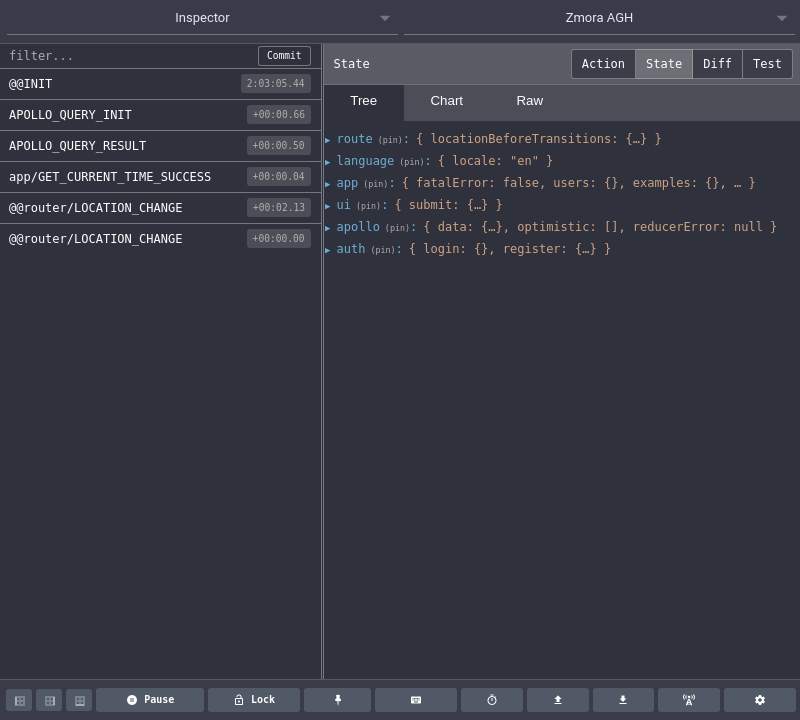
\includegraphics[width=0.9\textwidth]{images/redux_devtools}
	\caption{Okno dodatku Redux DevTools}
	\label{fig:reduxDevTools}
\end{figure}

